\section{Config Class Reference}
\label{classConfig}\index{Config@{Config}}
Inheritance diagram for Config::\begin{figure}[H]
\begin{center}
\leavevmode
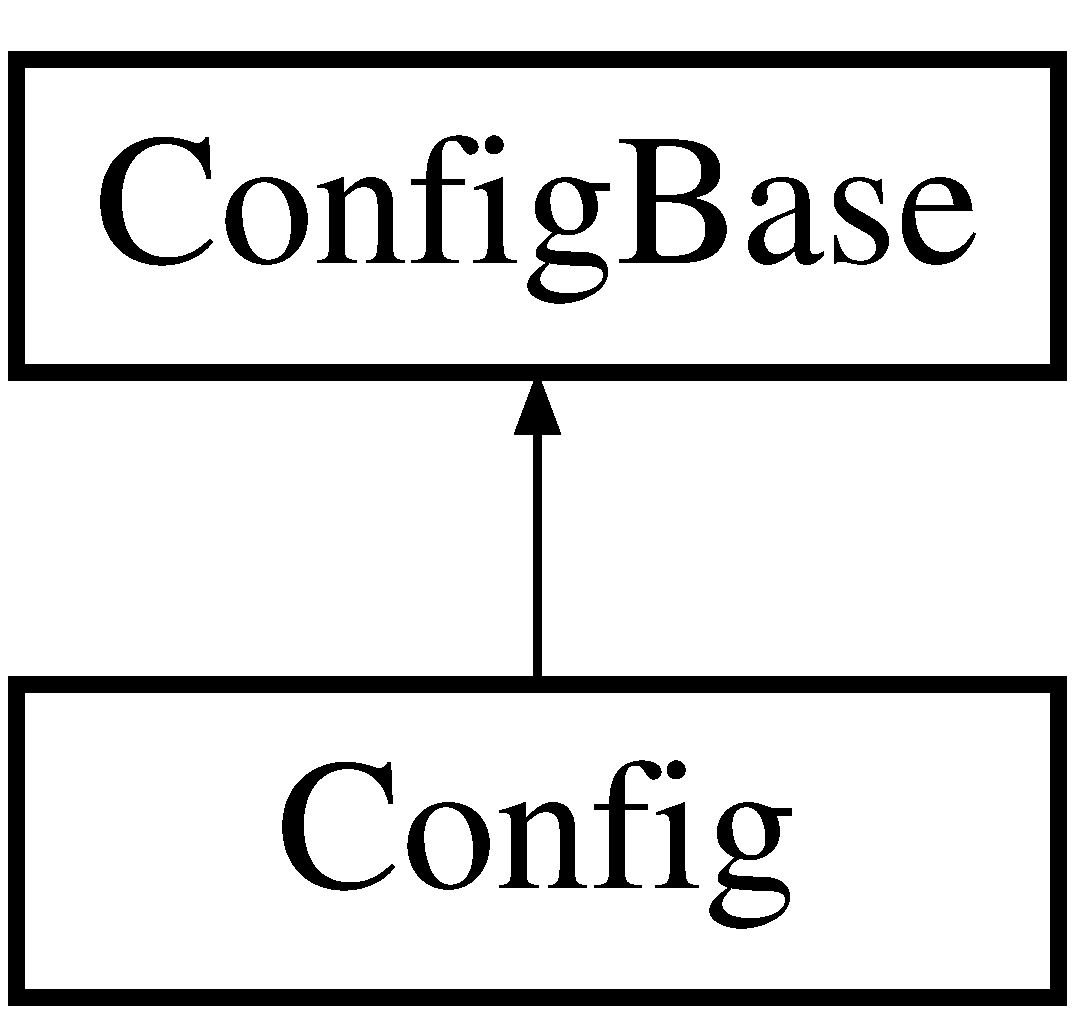
\includegraphics[height=2cm]{classConfig}
\end{center}
\end{figure}
\subsection*{Public Member Functions}
\begin{CompactItemize}
\item 
{\bf \_\-\_\-init\_\-\_\-} (name, var, def\_\-val, trans=None)
\item 
{\bf update} (val)
\item 
{\bf \_\-\_\-init\_\-\_\-} (name, def\_\-val)
\end{CompactItemize}


\subsection{Member Function Documentation}
\index{Config@{Config}!__init__@{\_\-\_\-init\_\-\_\-}}
\index{__init__@{\_\-\_\-init\_\-\_\-}!Config@{Config}}
\subsubsection{\setlength{\rightskip}{0pt plus 5cm}Config\-Base::\_\-\_\-init\_\-\_\- (name, def\_\-val)\hspace{0.3cm}{\tt  [inherited]}}\label{classConfigBase_ConfigBasea0}


\index{Config@{Config}!__init__@{\_\-\_\-init\_\-\_\-}}
\index{__init__@{\_\-\_\-init\_\-\_\-}!Config@{Config}}
\subsubsection{\setlength{\rightskip}{0pt plus 5cm}Config::\_\-\_\-init\_\-\_\- (name, var, def\_\-val, trans = {\tt None})}\label{classConfig_Configa0}


\index{Config@{Config}!update@{update}}
\index{update@{update}!Config@{Config}}
\subsubsection{\setlength{\rightskip}{0pt plus 5cm}Config::update (val)}\label{classConfig_Configa1}




Reimplemented from {\bf Config\-Base} {\rm (p.\,\pageref{classConfigBase_ConfigBasea1})}.

The documentation for this class was generated from the following file:\begin{CompactItemize}
\item 
{\bf Config\-Admin.py}\end{CompactItemize}
